
%(BEGIN_QUESTION)
% Copyright 2014, Tony R. Kuphaldt, released under the Creative Commons Attribution License (v 1.0)
% This means you may do almost anything with this work of mine, so long as you give me proper credit

The circuit shown here is commonly referred to as a {\it current divider}.  Calculate the voltage dropped across each resistor, the current drawn by each resistor, and the total amount of electrical resistance ``seen'' by the 9-volt battery:

$$\includegraphics[width=15.5cm]{i01147x01.eps}$$

\begin{itemize}
\item{} Current through the 2 k$\Omega$ resistor = 
\item{} Current through the 3 k$\Omega$ resistor = 
\item{} Current through the 5 k$\Omega$ resistor = 
\item{} Voltage across each resistor = 
\item{} $R_{total}$ = 
\end{itemize}

\underbar{file i01147}
%(END_QUESTION)





%(BEGIN_ANSWER)

\begin{itemize}
\item{} Current through the 2 k$\Omega$ resistor = 4.5 mA
\item{} Current through the 3 k$\Omega$ resistor = 3 mA
\item{} Current through the 5 k$\Omega$ resistor = 1.8 mA
\item{} Voltage across each resistor = 9 volts
\item{} $R_{total}$ = 967.74 $\Omega$
\end{itemize}

%(END_ANSWER)





%(BEGIN_NOTES)

Some students may find the diagram hard to follow, and so they will find the task of analysis helped by drawing an equivalent schematic diagram for this circuit, with all terminal points labeled.  I recommend you not suggest this solution immediately, but rather challenge your students to think of problem-solving techniques on their own.  Surely, someone in the class will have thought of doing this, and the impact of such a suggestion coming from a peer is greater than if it came from you, the instructor.

Be sure to ask your students this question: ``Why is this type of circuit commonly called a {\it current divider}?''

%INDEX% Electronics review: series and parallel circuits

%(END_NOTES)


